%%%%%%%%%%%%%%%%%%%%%%%%%%%%%%%%%%%%%
% Kindle diagnostic: a short book of labeled test cases for things that look
% different on a Kindle than in the PDF, a web browser or Calibre.
%
% Build with "tests/build_diagnostic.sh". It makes two epubs from the same HTML:
% kindle_diagnostic-raw.epub (make4ht output as it is) and kindle_diagnostic.epub
% (after lib/epub_postprocess.sh, as build.sh does for the book). Send both to a
% Kindle and compare the tests by ID.

\documentclass[pagesize=auto]{scrbook}

\usepackage{comment}
\usepackage{etoolbox}
\usepackage{fancyvrb}
\usepackage{graphicx}
\usepackage{hyperref}
\usepackage{makeidx}
\usepackage[round]{natbib}
\usepackage{xspace}
\usepackage{xcolor}

% This is for multilingual work. Would be nice to support Chinese and Thai.
\usepackage[T2A]{fontenc}
\usepackage[utf8]{inputenc}
\usepackage[greek,russian,english]{babel}
% This file is for commands / macros / functions. 
% Try to make sure that everything with a conditional such as \ifdefined\HCode goes in this file.

\newcommand{\latex}{\LaTeX\xspace}

\newcommand\nextpage[1][]{
\ifdefined\HCode {
  \HCode{<mbp:pagebreak />}}
\else
  % \newpage pdflatex leaves blank page anyway
\fi
}

\usepackage{amsmath}

\ifdefined\HCode{\KOMAoptions{twoside=false}} \fi

% Build stamp (date and git commit), written by build_diagnostic.sh.
\InputIfFileExists{kindle_diagnostic_stamp}{}{\def\kstamp{unstamped build}}

% A group of tests: a chapter, listed in the contents.
\newcommand{\kgroup}[1]{\chapter*{#1}\addcontentsline{toc}{chapter}{#1}}

% One test: ID, short name, status. Listed in the contents as a section.
\newcommand{\ktest}[3]{\section*{#1\quad #2\quad [#3]}\addcontentsline{toc}{section}{#1 #2}}

% What you see when the test works, and when it fails. Each test gives its
% source just before this, outside any macro argument, so that \sverb works.
\newcommand{\kcheck}[2]{\noindent\textbf{Good if:} #1\par
\noindent\textbf{Bad if:} #2\par}

% A paragraph with the test case twice, in mid-line, so that any change of
% baseline or line spacing shows against the lines around it.
\newcommand{\kpara}[1]{\par\smallskip\noindent This sentence is here to fill
a few lines of ordinary text around the test, which comes now: #1, and then
comes once more: #1, after which the sentence carries on for long enough to
make several full lines on a small screen, so their spacing can be compared
with the spacing of the paragraph in test A0.\par}

\begin{document}

\chapter*{Kindle Diagnostic}

\noindent Build: \kstamp

\medskip
\noindent This book comes in two versions with the same tests:
\textbf{raw} (make4ht output as it is) and \textbf{fixed} (after the
post-processing that \smalltt{build.sh} applies to the book). The epub title says
which one you are reading.

\medskip
\noindent Each test has an ID, a status, the source it uses, and two lines:
\textbf{Good if} (what you see when it works) and \textbf{Bad if} (what you see
when it is broken). Status labels:

\begin{itemize}
\item \textbf{[FIXED]} bad in the raw version, fixed by the build.
\item \textbf{[OPEN]} bad in both versions; no fix yet.
\item \textbf{[AVOID]} bad in both versions; write it a different way.
\item \textbf{[CHECK]} expected to work; still to be checked on a device.
\item \textbf{[REFERENCE]} a control to compare other tests with.
\end{itemize}

\noindent Check at two font sizes. Note results by ID and version, for
example \textit{A3 raised in raw, fine in fixed}.

\tableofcontents

%%%%%%%%%%%%%%%%%%%%%%%%%%%%%%%%%%%%%
\kgroup{A. Inline math}

\noindent Kindle sets every inline MathML formula in a small math font, raised
above the baseline, which spreads the lines around it. The build turns simple
inline math into ordinary italic text with subscripts and superscripts.

\ktest{A0}{Control: no math}{REFERENCE}
\noindent\textbf{Source:} \sverb|\emph{x}|.\par
\kcheck{this is the line spacing the other tests are compared with.}{(nothing; this is the control).}
\kpara{\emph{x}}

\ktest{A1}{Single letter}{FIXED}
\noindent\textbf{Source:} \sverb|$x$|.\par
\kcheck{the x sits on the line and the spacing matches A0.}{the x is raised or small, or the lines around it are spread apart.}
\kpara{$x$}

\ktest{A2}{Greek letter}{FIXED}
\noindent\textbf{Source:} \sverb|$\alpha$| (tex4ht writes the math italic character U+1D6FC).\par
\kcheck{an italic alpha on the line, spacing as in A0.}{a box instead of alpha, or a raised letter.}
\kpara{$\alpha$}

\ktest{A3}{Short expression}{FIXED}
\noindent\textbf{Source:} \sverb|$a + b = c$| and \sverb|$-1$|.\par
\kcheck{spaced operators, a minus sign close to its 1, everything on the line.}{raised or small text, or a gap between minus and 1.}
\kpara{$a + b = c$ and $-1$}

\ktest{A4}{Subscript and superscript}{FIXED}
\noindent\textbf{Source:} \sverb|$x_i^2$| and \sverb|$e^{-n}$|.\par
\kcheck{the lines spread apart only a little, as with any superscript.}{the lines spread apart a lot.}
\kpara{$x_i^2$ and $e^{-n}$}

\ktest{A5}{Fraction and square root}{FIXED}
\noindent\textbf{Source:} \sverb|$\frac{a+b}{2}$| and \sverb|$\sqrt{n+1}$|.\par
\kcheck{(a + b)/2 and a radical sign with brackets, on the line.}{a small stacked fraction, or a raised formula.}
\kpara{$\frac{a+b}{2}$ and $\sqrt{n+1}$}

\ktest{A6}{Bold and script letters}{FIXED}
\noindent\textbf{Source:} \sverb|$\mathbf{v}$| and \sverb|$\mathcal{F}$|.\par
\kcheck{a bold v and a curly script F, on the line.}{plain letters, a box, or a raised formula.}
\kpara{$\mathbf{v}$ and $\mathcal{F}$}

\ktest{A7}{Accent}{AVOID}
\noindent\textbf{Source:} \sverb|$\hat{x}$|. Accents stay MathML in the fixed version too.\par
\kcheck{an x with a hat, on the line.}{the formula is raised, or the hat is misplaced (expected in both versions).}
\kpara{$\hat{x}$}

\ktest{A8}{Symbols written as text, not math}{CHECK}
\noindent\textbf{Source:} \sverb|\texttimes| and \sverb|\textsubscript{2}| in ordinary text, no math mode.\par
\kcheck{a times sign and a subscript 2, spacing as in A0, in both versions.}{a box instead of the times sign.}
\kpara{3\texttimes{}4 and H\textsubscript{2}O}

%%%%%%%%%%%%%%%%%%%%%%%%%%%%%%%%%%%%%
\kgroup{B. Matrices and brackets}

\noindent tex4ht writes an empty \smalltt{rowlines} attribute on every MathML
table, which Kindle draws as rules between the rows. The build sets these to
\smalltt{none}.

\ktest{B1}{pmatrix}{FIXED}
\noindent\textbf{Source:} \sverb|\begin{pmatrix}...\end{pmatrix}|.\par
\kcheck{a clean matrix in round brackets.}{horizontal lines between or around the rows.}
\[
\begin{pmatrix}
  1 & 2 & 3 \\
  4 & 5 & 6 \\
\end{pmatrix}
\]

\ktest{B2}{array inside left and right brackets}{FIXED}
\noindent\textbf{Source:} \sverb|\left(\begin{array}{cc}...\end{array}\right)|.\par
\kcheck{a clean matrix in round brackets.}{horizontal lines between the rows.}
\[
\left(
\begin{array}{cc}
a & -b \\
b & a
\end{array}
\right)
\]

\ktest{B3}{bmatrix}{FIXED}
\noindent\textbf{Source:} \sverb|\begin{bmatrix}...\end{bmatrix}|.\par
\kcheck{a clean matrix in square brackets.}{horizontal lines, or round brackets.}
\[
\begin{bmatrix}
0 & 1 \\
1 & 0 \\
\end{bmatrix}
\]

\ktest{B4}{Big brackets}{CHECK}
\noindent\textbf{Source:} \sverb|\bigl(| \ldots\ \sverb|\bigr)|. The build makes them stretchy, like \sverb|\left(|.\par
\kcheck{tall brackets, centered on the fraction they enclose.}{small brackets, or brackets sitting low on the baseline.}
\[
f\bigl(\tfrac{1}{2}\bigr) = \Bigl(\frac{a}{b}\Bigr)^2
\]

%%%%%%%%%%%%%%%%%%%%%%%%%%%%%%%%%%%%%
\kgroup{C. Display math and equation links}

\ktest{C1}{Numbered equation and a link to it}{OPEN}
\noindent\textbf{Source:} \sverb|\begin{equation}\label{...}| and \sverb|Equation~\ref{...}|.\par
\kcheck{tapping the link below jumps to the equation.}{the link does nothing (expected: the link target sits inside the MathML, and Kindle Previewer reports it as unresolved).}
\begin{equation}
y = m x + c
\label{eq:kdiag}
\end{equation}
Tap this link: Equation~\ref{eq:kdiag}.

\ktest{C2}{Aligned equations}{CHECK}
\noindent\textbf{Source:} \sverb|\begin{align*}|.\par
\kcheck{the equals signs line up; the fraction and square root are drawn properly.}{rows out of line, or a broken fraction or square root.}
\begin{align*}
s &= \sqrt{a^2 + b^2} \\
t &= \frac{a + b}{a - b}
\end{align*}

%%%%%%%%%%%%%%%%%%%%%%%%%%%%%%%%%%%%%
\kgroup{D. Footnotes}

\noindent Kindle shows a footnote as a pop-up only when the marker links to the
note and the note links back to the marker. tex4ht makes only the first link;
the build adds the link back.

\ktest{D1}{Footnote}{FIXED}
\noindent\textbf{Source:} \sverb|\footnote{...}|.\par
\kcheck{tapping the number shows the note in a pop-up.}{tapping the number jumps to the end of the book.}
\par\smallskip\noindent This sentence makes a claim that needs a short note.\footnote{This is the note. Without pop-ups it is read as an endnote, so it should make sense on its own.} The paragraph then goes on for a while, so the marker sits in the middle of a paragraph.

%%%%%%%%%%%%%%%%%%%%%%%%%%%%%%%%%%%%%
\kgroup{E. Contents page}

\ktest{E1}{Contents spacing}{FIXED}
\noindent\textbf{Source:} \sverb|\tableofcontents|, at the start of this book.\par
\kcheck{one entry per line, chapters in bold, tests indented, no blank lines between entries.}{a blank line between every pair of entries.}

%%%%%%%%%%%%%%%%%%%%%%%%%%%%%%%%%%%%%
\kgroup{F. Figures and captions}

\noindent tex4ht turns image widths into a fixed size in pixels, so images
come out small on a Kindle. \smalltt{lib/ebook-layout.cfg} turns them into a
percentage of the screen width instead. That file is used for both versions.

\ktest{F1}{Full-width figure}{CHECK}
\noindent\textbf{Source:} \sverb|\includegraphics[width=\linewidth]| in a \sverb|figure| with a caption.\par
\kcheck{the map fills the width of the text; the caption is about as wide as the text.}{a small map, or a narrow, tall caption.}
\begin{figure}[ht]
\centering
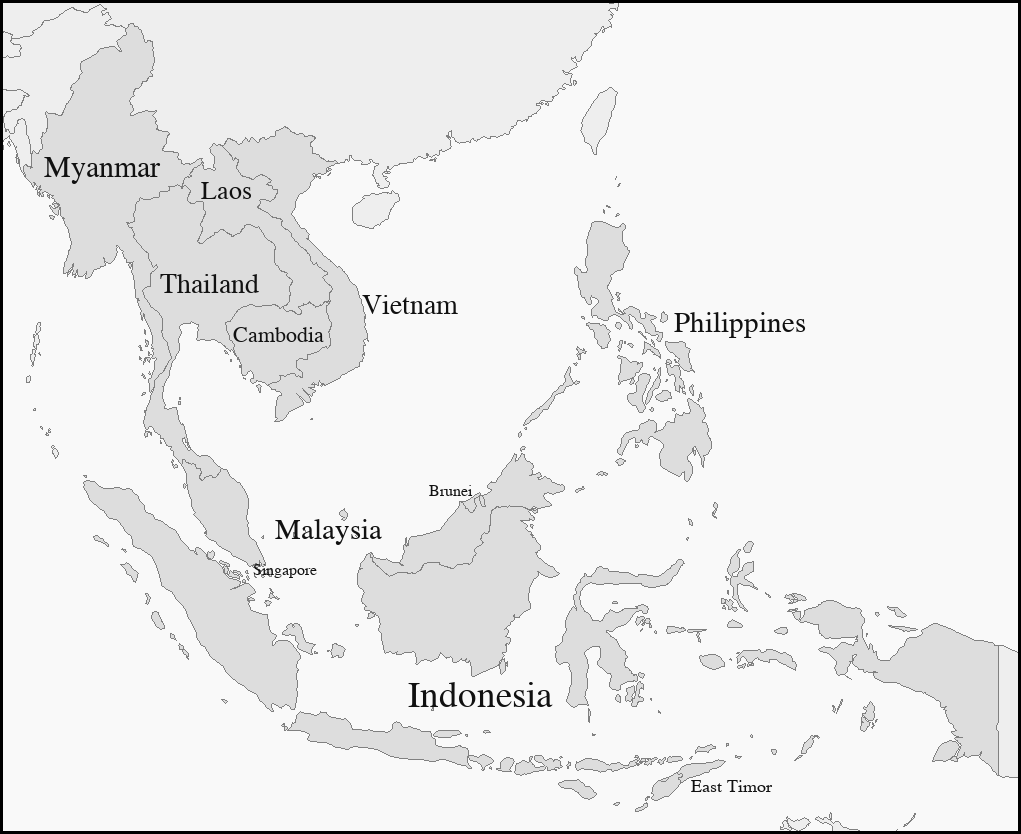
\includegraphics[width=\linewidth]{images/sea_countries.png}
\caption{A long caption, so that its width is easy to judge against the text above. It should run nearly the full width of the screen.}
\end{figure}

\ktest{F2}{Half-width figure}{CHECK}
\noindent\textbf{Source:} \sverb|\includegraphics[width=0.5\linewidth]|.\par
\kcheck{the map fills half the width of the text; the caption is as wide as in F1.}{the map is much smaller than half, or the caption is narrower than in F1.}
\begin{figure}[ht]
\centering
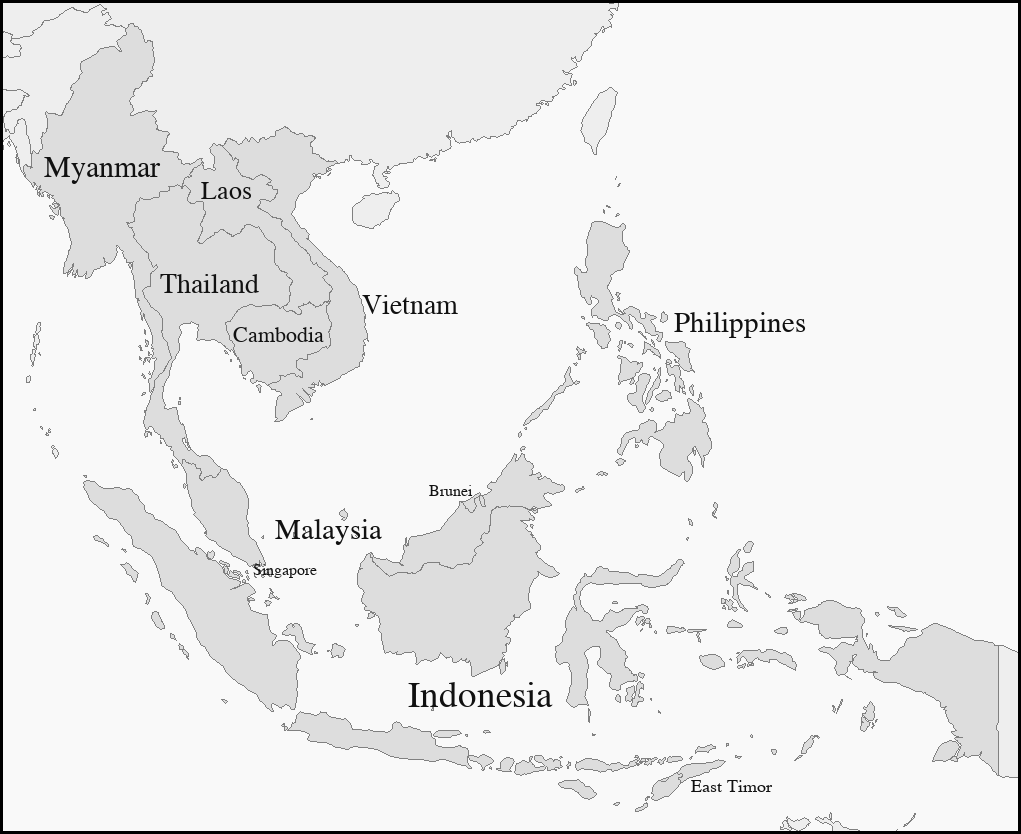
\includegraphics[width=0.5\linewidth]{images/sea_countries.png}
\caption{A long caption, so that its width is easy to judge against the text above. It should run nearly the full width of the screen.}
\end{figure}

\ktest{F3}{Fixed width}{CHECK}
\noindent\textbf{Source:} \sverb|\includegraphics[width=4cm]|.\par
\kcheck{the map is a little under a third of the text width (4cm of the PDF's text width).}{a tiny map.}
\begin{center}
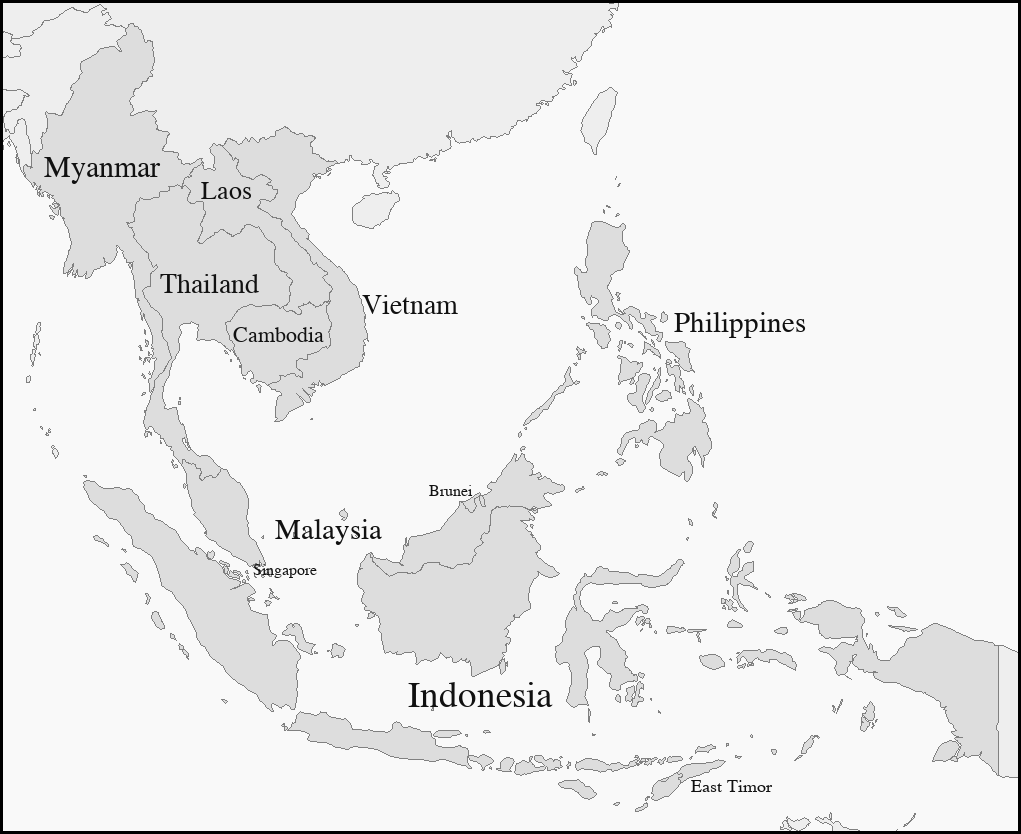
\includegraphics[width=4cm]{images/sea_countries.png}
\end{center}

%%%%%%%%%%%%%%%%%%%%%%%%%%%%%%%%%%%%%
\kgroup{G. Text features}

\ktest{G1}{Code listing width}{CHECK}
\noindent\textbf{Source:} \sverb|\begin{Verbatim}|. The first line is a ruler of 60 characters.\par
\kcheck{the 52-character line fits on one line and its indentation is kept (also note the last ruler digit that fits).}{the 52-character line wraps, or the indentation is lost.}
\begin{Verbatim}
123456789.123456789.123456789.123456789.123456789.123456789.
    for word in sorted(counts, key=counts.get):
        print(f"{word:>20} {counts[word]:6d}")
\end{Verbatim}

\ktest{G2}{Table with rules}{CHECK}
\noindent\textbf{Source:} \sverb!\begin{tabular}{|c|l|}! with \sverb|\hline|.\par
\kcheck{a border around the table and one line under the header row.}{missing or extra lines.}
\begin{center}
\begin{tabular}{|c|l|}
\hline
\textbf{Format} & \textbf{Used for} \\
\hline
PDF & print and screen \\
EPUB & eReaders \\
\hline
\end{tabular}
\end{center}

\ktest{G3}{Small typewriter text}{CHECK}
\noindent\textbf{Source:} \sverb|\smalltt{...}| and \sverb|\sverb|.\par
\kcheck{monospace text, slightly smaller than the body text.}{the body font, or much smaller text.}
\kpara{\smalltt{build.sh}}

%%%%%%%%%%%%%%%%%%%%%%%%%%%%%%%%%%%%%
\kgroup{H. Other languages}

\ktest{H1}{Greek and Russian through babel}{CHECK}
\noindent\textbf{Source:} \sverb|\foreignlanguage{greek}{...}| and \sverb|\foreignlanguage{russian}{...}| around UTF-8 text.\par
\kcheck{all the letters and accents appear, on the line, with even spacing.}{boxes, missing accents, or uneven spacing.}
\kpara{\foreignlanguage{greek}{βιβλίο} and \foreignlanguage{russian}{книга}}

\ktest{H2}{Greek spelled with math letters}{AVOID}
\noindent\textbf{Source:} \sverb|$\beta\iota\beta\lambda\iota o$|. Use babel as in H1 instead.\par
\kcheck{(not expected).}{in the raw version, raised letters; in the fixed version, italic letters with no accents.}
\kpara{$\beta\iota\beta\lambda\iota o$}

\end{document}
